\documentclass{crm-article}

%\usepackage{parskip} %for leaving some space after paragraphs
%\usepackage{mathtools} %for begin equation
%\usepackage{authblk} %authors and their affiliations
%\usepackage{graphicx} %for include graphics
%\usepackage{subcaption}
\usepackage{float} %to not make images float around
\graphicspath{{figures/}}

\begin{document}
	\englishpaper
	\norussian

	\journalVol{10}
	\journalNo{2}
	\setcounter{page}{1}
	\journalSection{Mathematical modeling and numerical simulation}

	\journalReceived{11.10.2023.}
	%\journalReviewed{01.06.2016.}
	\journalAccepted{11.12.2023.}

	\UDC{532.685}
	\title{Simulation of Imbibition for Two-Phase Flow in Porous Media using a Two-Dimensional Network Model}
	\thanks{This project was supported by grant 23-21-00175 of Russian Science Foundation, \url{https://rscf.ru/project/23-21-00175/}}

	\author{\firstname{K.}~\surname{Shabbir}}
	\authorfull{Kafi Ul Shabbir}
	\email{kafiulshabbir@phystech.edu}
	\affiliation{Moscow Institute of Physics and Technology,\protect\\ 9 Institutskiy pereulok, Dolgoprudny, Moscow Region, 141700, Russia}

	% repeat for the rest authors,
	% skip \affiliation if it is already listed above
	% if automatic reference generation does not provide correct results
	% state the correct numbers in square brackets
	
	\author[1]{\firstname{O.\,Ya.}~\surname{Izvekov}}
	\authorfull{Oleg Ya. Izvekov}
	\email{izvekov\_o@inbox.ru}
	
	\author{\firstname{A.\,V.}~\surname{Konyukhov}}
	\authorfull{Andrey V. Konyukhov}
	\email{konyukhov\_av@mail.ru}
	\affiliation{Joint Institute for High Temperatures of the Russian Academy of Sciences,\protect\\ 13/2 Izhorskaya st., Moscow, 125412, Russia}


	\begin{abstract}
		Simulation of two-phase flow in porous media has many applications in oil recovery, hydrology, electricity production, etc. Classical continuum models consider permeability to be a function of only saturation. Classical continuum models are unable to explain non-equilibrium effects. Advanced continuum models, such as the Kondaurov model considers permeability to be a function of a non-equilibrium parameter in addition to saturation. In order to better understand the non-equilibrium effects, it is necessary to develop non-continuum models at the scale of the pores, for example a network model. The objective of our research is to understand the physical meaning of the Kondaurov non-equilibrium parameter. In this article, we describe the network model we developed for simulating two-phase flow in porous media. At first we determine the pressures in each node by solving a system of linear equations. Then from the known pressures we calculate the flow rates. Lastly we decide an appropriate time step, distribute the fluids in the nodes, and perform displacement of the fluids in the tubes. Our model uses a novel method of distributing different phases in the nodes. We simulated the process of imbibition, where wetting fluid was located in the outer region with thicker radius, and non-wetting fluid in the inner region with thinner radius or finer pores. We measured the saturation of the wetting phase with respect to time in the region of finer pores. Our network model successfully shows that the wetting fluid invades the region of finer pores, and the saturation with respect to time rests to an equilibrium value. 
	\end{abstract}
	
	\keyword{Capillary pressure}
	\keyword{non-equilibrium effect}
	\keyword{advanced continuum model}
	\keyword{Hagen–Poiseuille equation}
	\keyword{laminar flow}
	\keyword{meniscus}
	\keyword{viscosity}
	\keyword{fluid displacement}

	\maketitle
	
	\section{Introduction} \label{sec:intro}
		Simulation of two-phase flow in porous media has applications in oil recovery, hydrology, electricity production where pressurized water is passed through heated pipes and is transformed into steam, etc. Hence it is important to understand and model two-phase flow in porous medium. \cite{labed2012experimental}
			
		\subsection{Classical continuum models}

			Classical continuum models are widespread and useful. Darcy's Law is an example of classical continuum model. It is given by:
			
			\begin{gather}
				q = -\frac{k}{\mu} \nabla p
				\label{eq:basic-darcy}
			\end{gather}
			
			Here, $q$ is the flow rate,	$k$ is the permeability, $\mu$ is the coefficient of viscosity,	and $\nabla p$ is the pressure gradient.
			
			The feature of these classical continuum models is that the permeability is only a function of the saturation of one of the phase.
			\begin{gather}
				k = k(S)
			\end{gather}
			
			Here, $k$ is the permeability as in equation \ref{eq:basic-darcy}, and $S$ is the saturation of one of the phase.

			Saturation $S$ is defined as the ratio between the volume occupied by a phase to the total volume of the void. For wetting phase,

			\begin{gather}
				S_{w} = \frac{V_{w}}{V_{void}}
			\end{gather}
			
			Here, $V_{w}$ is volume occupied by the wetting phase, $V_{void}$ is total volume of the void. For non-wetting phase,
			
			\begin{gather}
				S_{nw} = \frac{V_{nw}}{V_{void}}
			\end{gather}
			
			It is clear that,
			
			\begin{gather}
				S_{w} + S_{nw} = 1
			\end{gather}
			
			In this article, we denote $S$ to be the saturation of the wetting phase.
			
		\subsection{Advanced continuum models}
			The classical continuum models are valid as long as the characteristic time of the processes is much longer than the characteristic time of fluid redistribution in the capillary space.
			
			The characteristic time can be longer due to non-equilibrium effects, which occurs when the saturation changes rapidly, or the porous medium is a fractured one with blocks and cracks. In these cases, the assumption that $k = k(S)$ is not sufficient and additional parameters are required.

			Various advanced continuum models that take such non-equilibrium effects into account. Models of Hassanizadeh \cite{hassanizadeh2004continuum} \cite{hassanizadeh1987high} and Barenblatt \cite{barenblatt1960basic} consider that, the permeability $k$ is a function of the rate of saturation change, in addition to the saturation $S$.                  
			
			\begin{gather}
				k = k(S, \frac{\partial S}{\partial t})
			\end{gather}
			
			Here,
			
			\begin{gather}
				S = S(t)
			\end{gather}
			
			The Kondaurov model \cite{kondaurov2009non} considers a special non-equilibrium parameter $\xi$ along with saturation $S$, which relaxes to an equilibrium value. \cite{kondaurov2007thermodynamically}
			
			\begin{gather}
				k = k(S, \xi)
			\end{gather}
			
			This parameter $\xi$ is related to $S$ by the differential equation:
			
			\begin{gather}
				\frac{\partial \xi}{\partial t} = \Omega ( S, \xi )
			\end{gather}
			
			The objective of our research is to develop a network model which helps us better understand the Kondaurov non-equilibrium parameter $\xi$.
			 
		\subsection{Non-continuum models}
			In order to better understand the non-equilibrium characteristics, it is often necessary to simulate the flow at the scale of pores. Some of the methods of modeling at the scale of pores are, Lattice Boltzmann Method, a direct Navier-Stokes simulation, or a network model. Direct Navier-Stokes simulation provides very accurate results on velocity and pressure distributions, but it is very complicated. Network models are much simpler.
			
			One of the earliest models simulated the flow using a network of electrical resistors \cite{fatt1956network}. Some of the modern models, such as by Aker et al \cite{aker1998two} used an hour glass shaped model of tubes  to perform simulation, where the average flow rate was given by the Washburn equation for capillary flow \cite{washburn1921dynamics}. The disadvantage is that the flow rate must be approximated for cylindrical tube while in their model, the capillary pressure varied depending on its position in the tube.
			
			Our network model uses a novel method of distributing different phases at the nodes. It used only cylindrical tubes, and the flow rate is given by simple equations. In this article we demonstrate the applicability of our model by simulating imbibition.
			
		\subsection{Content of this article}
			\textbf{Section \ref{sec:model}} is about the physics of our network model.
			
			In section \ref{sec:approx-porous-medium}, we describe how we represent different properties of a porous media by a network model.
			
			Our algorithm for simulation:
			\begin{itemize}
				\item We generate a set of linear equations with pressure as the variables, section \ref{sec:linear-equ}.
				
				\item From the calculated pressure in each node, we determine the flow rate in each of the tubes, as shown in section \ref{sec:flow-rate-vel}.
				
				\item The phases are distributed in each of the nodes according to section \ref{sec:multi-phase-flow}.
				
				\item In order to constrain our data, we recombine phases in a capillary, when there are more than 2 menisci in a tube according to section \ref{sec:recombination-details}.
			\end{itemize}
			
			The details of how we derived the equations of flow rate with 1 meniscus is given in section \ref{sec:simple-flow-rate} and with multiple menisci in section \ref{sec:multi-menisci-flow-rate}.
			
			\textbf{Section \ref{sec:computation}} is about the various computational algorithms, methods, and problems we encountered along with their solutions. 
			
			The algorithm of simulation is detailed in section \ref{sec:detailed-algorithm}. Then we modeled the process of filtration with open boundaries in section \ref{sec:model-filtration} to check the validity of our model. For closed boundaries, we show that the system as infinitely many solutions in section \ref{sec:closed-boundary-triangle}. We then show an example of how our model behaves when a meniscus reaches a node in section \ref{sec:example-meniscus-in-node}.
			
			\textbf{Section \ref{sec:experiment}} is about our main experiment which the simulation of imbibition.
			
			The initial conditions in section \ref{sec:exp-init}. The type of computer we used, how the fluid distribution looked like in section \ref{sec:exp-main}. The results discussed in section \ref{sec:exp-discussion}.
			
			\textbf{Section \ref{sec:conclusion}} are some of the important conclusions.
	
		
	\section{Characteristics of the model} \label{sec:model}	
		\subsection{Approximation of a porous medium} \label{sec:approx-porous-medium}

		\begin{figure}[H]
			\centering
			\subfloat[Pore as node, and capillary as tube. \label{fig:descp-of-model}]{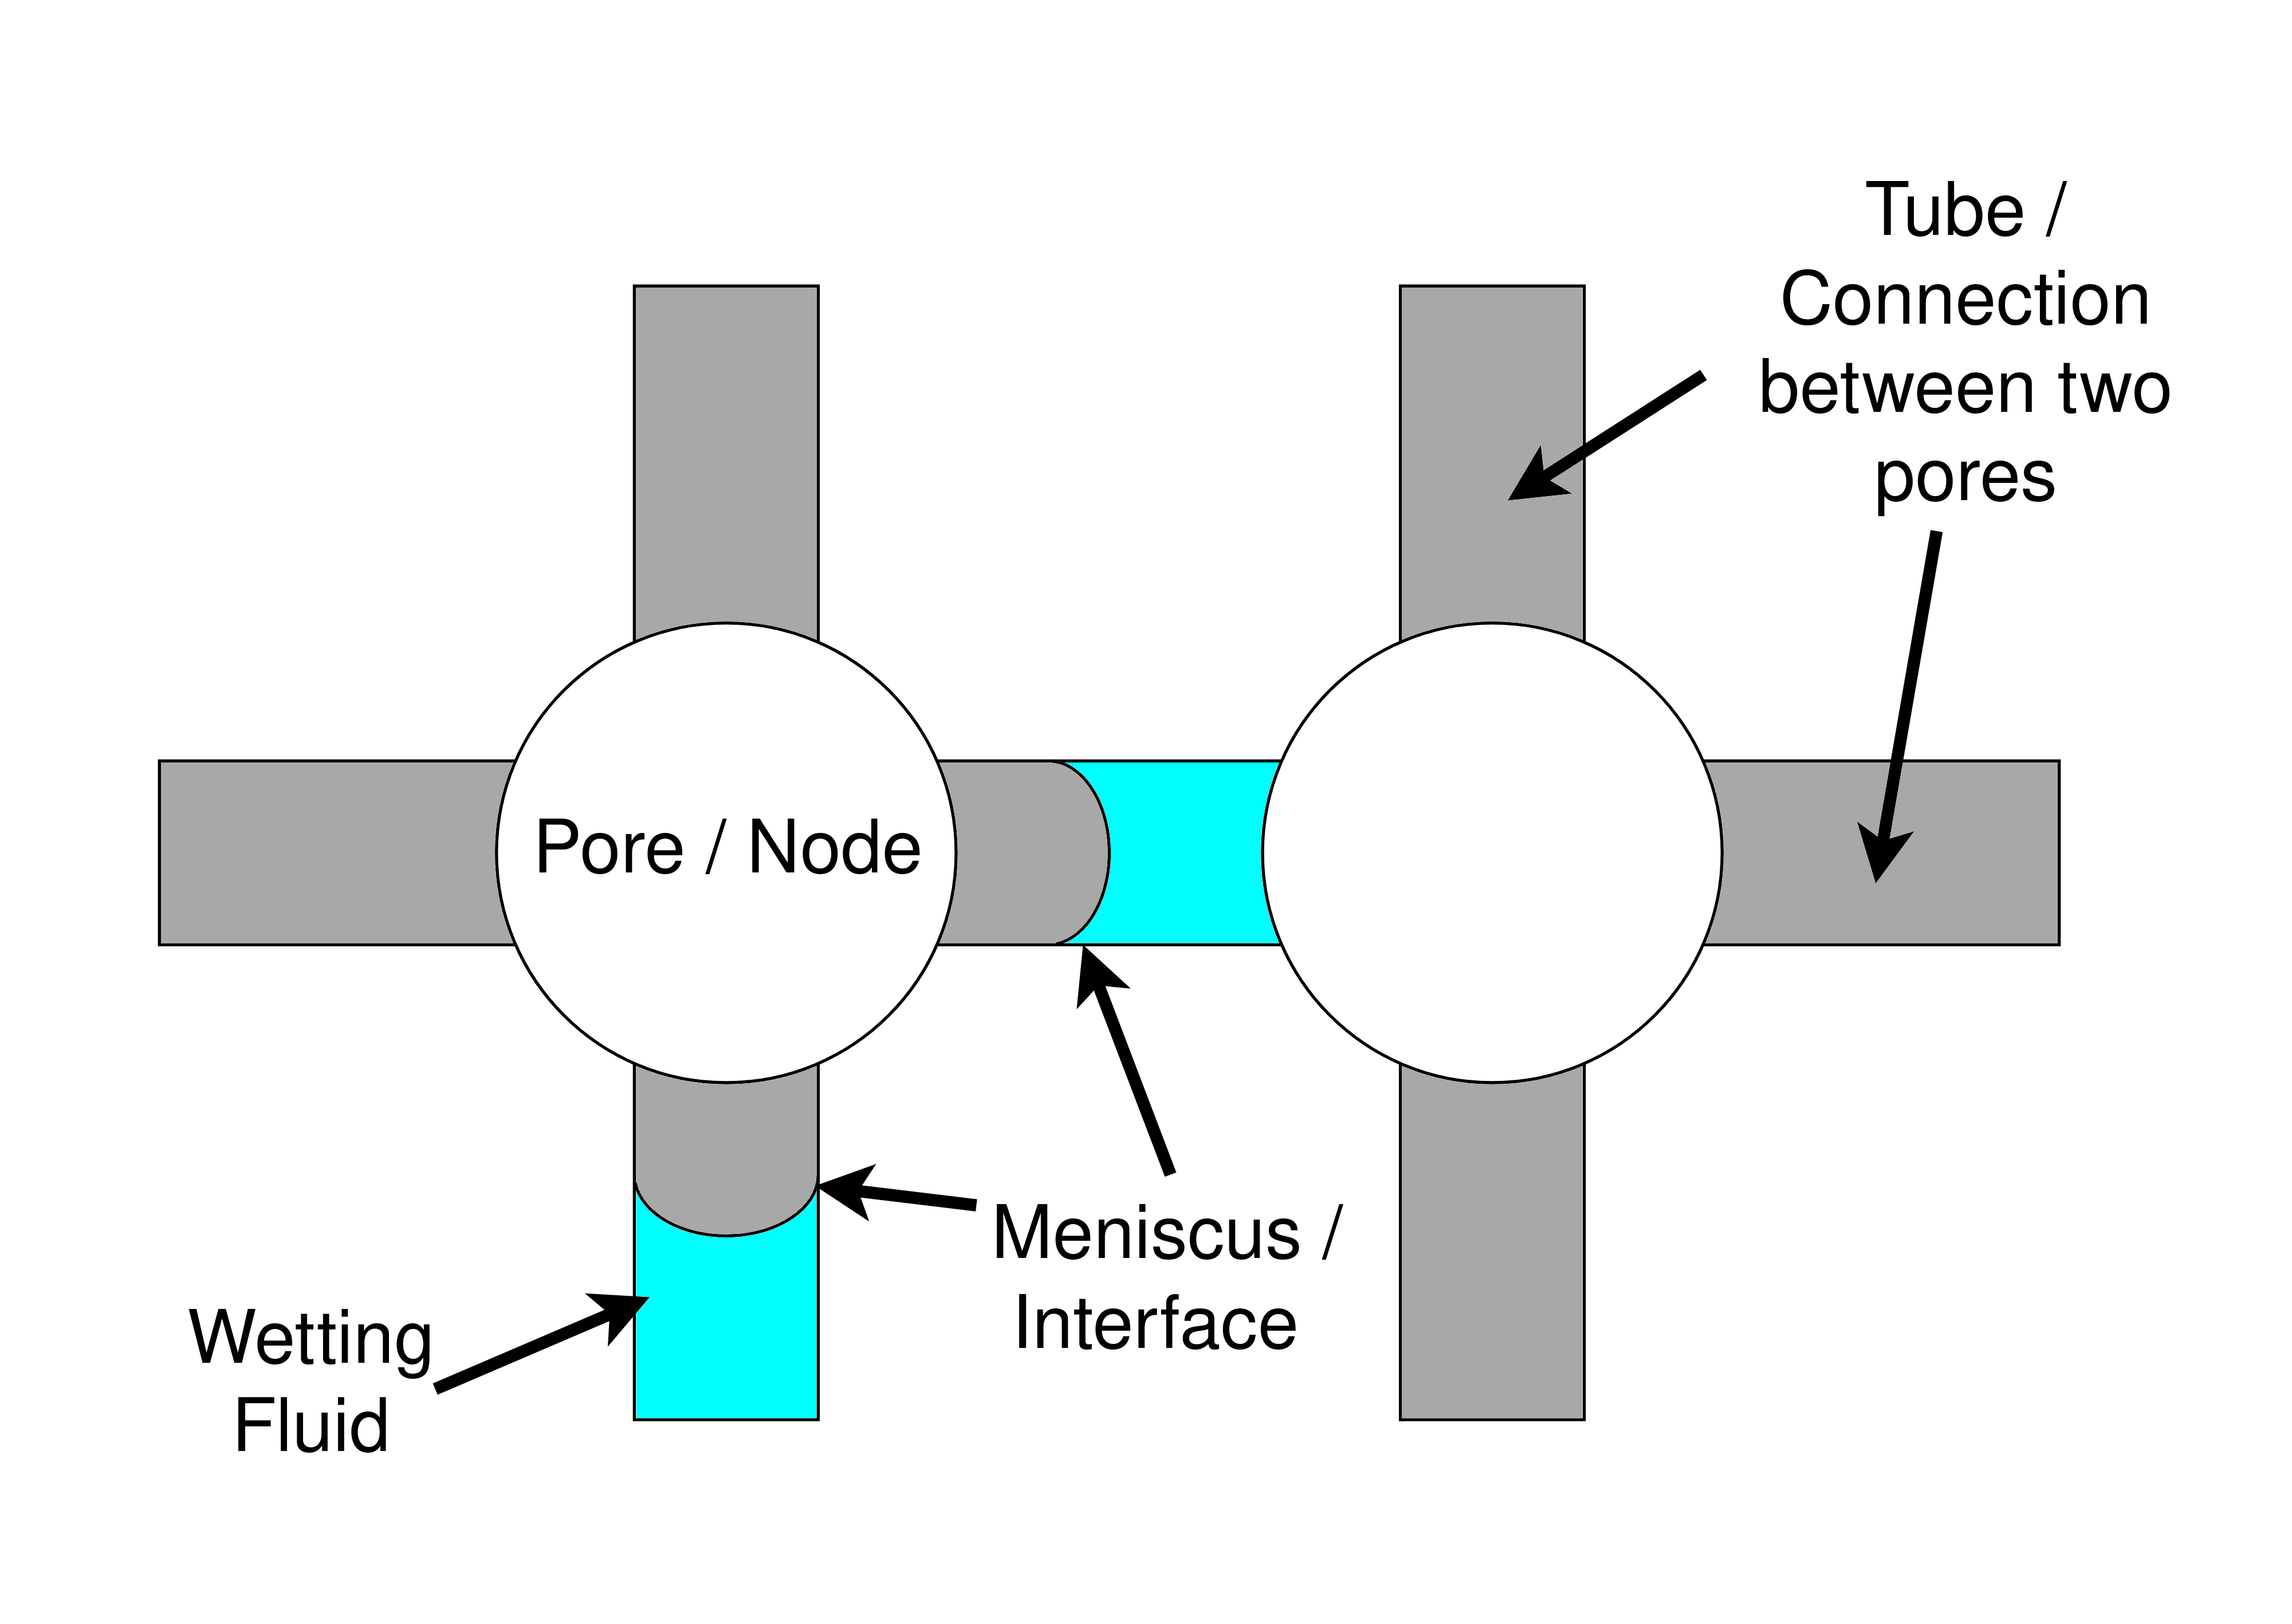
\includegraphics[width=0.55\textwidth]{fig_descp-of-model}}
			\subfloat[Flow rates in tubes connected to a node. \label{fig:simple-5-nodes}]{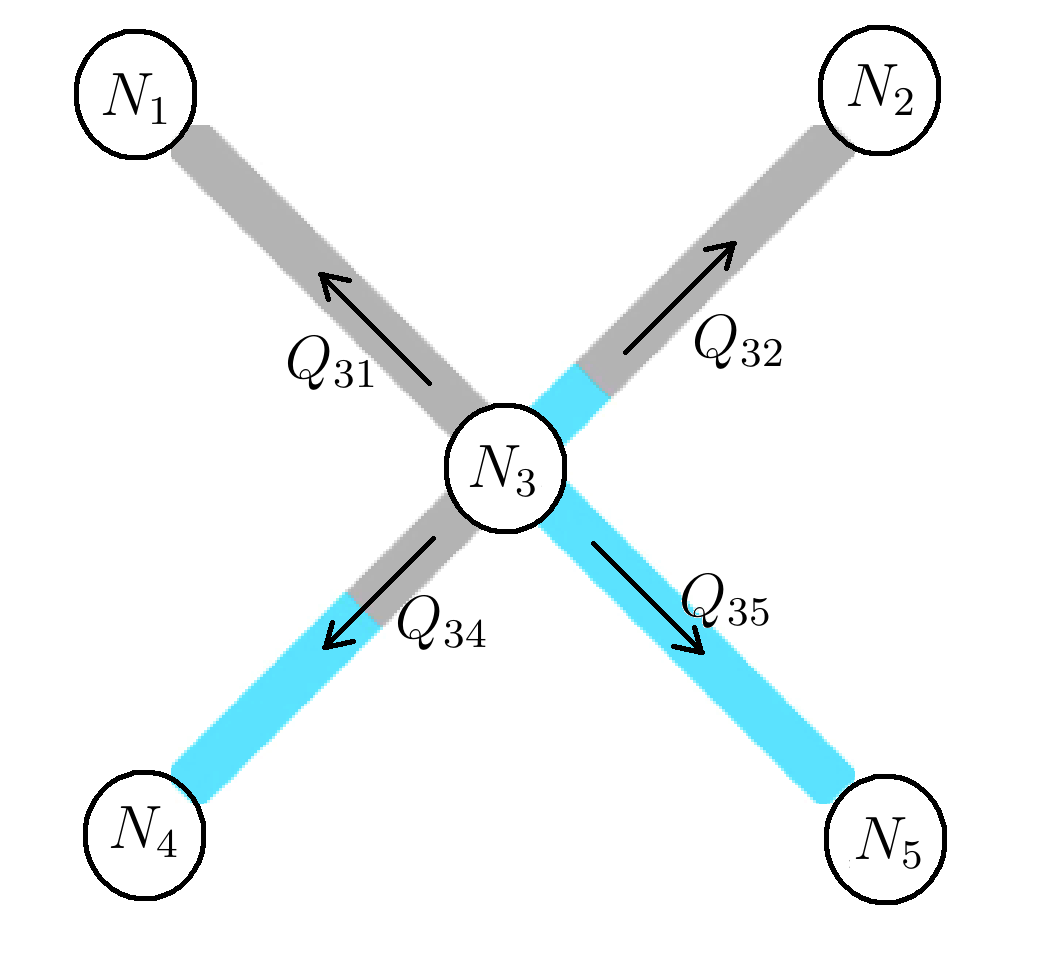
\includegraphics[width=0.4\textwidth]{fig_simple-5-nodes}}
			\caption{Network model of porous medium.}
		\end{figure}
		
		A porous medium consists of pores, which are connected by capillaries. The pores are represented by nodes, while the capillaries are represented by tubes, as shown in figure \ref{fig:descp-of-model}.
		
		Denotations for our model:
		
		\begin{itemize}
			\item Our model is two-dimensional 
			\item Each node is connected to 4 other nodes through tubes, shown in figure \ref{fig:simple-5-nodes}. They may be connected to less than 4 nodes, when they are located on the boundaries.
			\item The color cyan denotes wetting fluid, while the color gray denotes non-wetting fluid.
		\end{itemize}
		
		Assumptions:
		
		\begin{itemize}
			\item Gravity is ignored.
			\item The fluids are not compressible.
			\item The volume of the node is not taken into consideration and is assumed to be zero.
			\item All tubes are of equal length and cylindrical. The tubes can have different radii.
			\item The capillary pressure is zero inside the node.
			\item A tube can have a maximum of 2 menisci.
			\item During flow, when both cyan and gray fluid enters one node, then the fluids are distributed such that the cyan fluid is distributed first to the thinner tubes.
			\item During flow, if a tube has more than two meniscus, then there are combined together such that the center of mass of each fluid remains the same.
		\end{itemize}
		
		Note that the assumption of zero volume of node would not change the mixing of different fluids. Let us assume that a node with non-zero volume is filled with gray fluid is invaded by cyan fluid. Since the cyan fluid is distributed first, it immediately reaches the ends of the other tubes connected to the node. The assumption of zero volume of node only affects how the saturation is calculated, never the less it was assumed to be zero to keep the calculations for the flow simple.

	\subsection{Set of linear equations for a node} \label{sec:linear-equ}
		
		Let the flow rate in a tube be given by,
		\begin{gather}  \label{eq:flow-rate-simple-coeff}
			Q_{ij} = A_{ij}\Delta P_{ij} + B_{ij}
		\end{gather}
		
		Here, $Q_{ij}$ is the flow rate form node $N_i$ to node $N_i$. $A_{ij}$ and $B_{ij}$ are real constants. Here $\Delta P_{ij} = P_i - P_j$, where $N_i$ is kept at a pressure of $P_i$ and $N_j$ at a pressure of $P_j$. The detailed form is given by equation \ref{eq:main-flow-rate-with-s}
		
		During simulation, we produce a set of linear equations. We iterate through each node, write equations of flow rates for each tube connected to the node, and equate the sum to zero. For each node, we get one linear equation. For figure\ref{fig:simple-5-nodes}:
		
		\begin{gather}
			Q_{3j} = A_{3j}\Delta P_{3j} + B_{3j}
		\end{gather}

		Due to the conservation of volume, we have:
		\begin{gather}
			\sum_{k} Q_{3k} = 0
		\end{gather}
		
		Where $k = {1, 2, 4, 5}$.
		
		Note that all $Q$'s point outward. The $Q$'s will have different signs in order to preserve the law of conservation of volume. 
		
		For fluid flowing out of $N_3$,
		\begin{gather}
			Q_{3j} > 0
		\end{gather}
		
		For fluid flowing into $N_3$,
		\begin{gather}
			Q_{3j} < 0
		\end{gather}
		
		Let us assume that the pressures at all nodes are known, except $N_3$. Then, the set of linear equations is:
		
		\begin{gather} \label{eq:matrix-open-sys-5-nodes}
			\begin{pmatrix}
				1 & 0 & 0 & 0 & 0 & P_{1}\\
				0 & 1 & 0 & 0 & 0 & P_{2}\\
				-A_{31} & -A_{32} & (A_{31} + ... + A_{35}) & -A_{34} & -A_{35} & -(B_{31} + ... + B_{35})\\
				0 & 0 & 0 & 1 & 0 & P_{4}\\
				0 & 0 & 0 & 0 & 1 & P_{5}
			\end{pmatrix}
		\end{gather}
		
	\subsection{Multi-phase flow in a node} \label{sec:multi-phase-flow}
		The novelty of our model is how we distribute phases in the nodes. When more than one phase flows into a node, the wetting fluid first enters the tube with the thinner radius. This is to minimize the energy of the system. Below is an example:
		
		\begin{figure}[H]
			\centering
			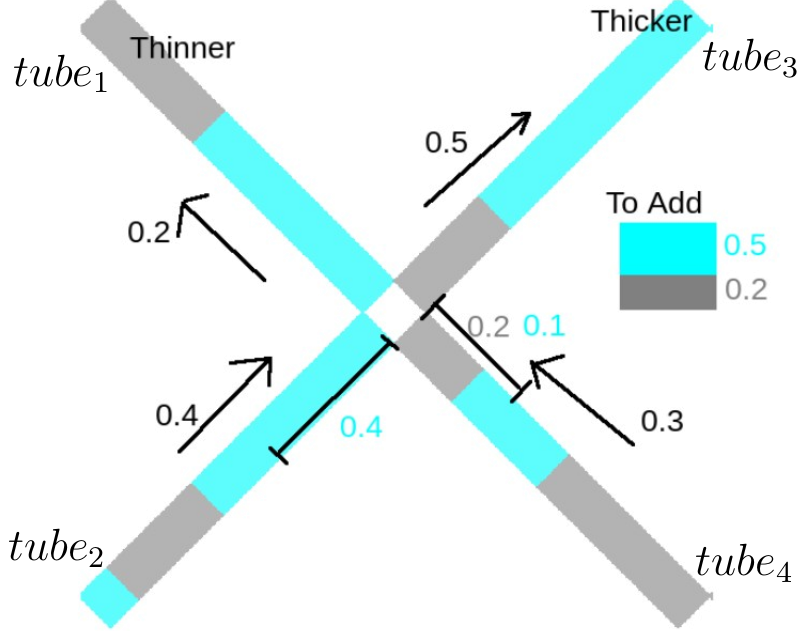
\includegraphics[width=0.45\textwidth]{fig_distributing_phases_initial}
			\caption{Distribution prediction of different fluids in a node.}
			\label{fig:distributing_phases_initial}
		\end{figure}
		
		In figure \ref{fig:distributing_phases_initial}, fluid flows from ${tube}_2$ and ${tube}_4$ into ${tube}_1$ and ${tube}_3$. 

		From the calculation of flow rates, we determined that $0.7 u.v.$ (unit volumes) of fluid enters the node, while $0.7 u.v.$ exits the node. They must be equal due to Kirchhoff's law at the node. The total inflow of $0.7 u.v.$ consists of $0.4 u.v.$ from ${tube}_2$ and $0.3 u.v.$ from ${tube}_4$. The outflow consists of $0.2 u.v.$ into ${tube}_1$, and $0.5 u.v.$ into ${tube}_3$.
		
		Step-1, we calculate the sum of volume of each type of fluid flowing into the node. Here, ${tube}_2$ provides $0.4 u.v.$ of cyan fluid, while ${tube}_4$ provides $0.1 u.v.$ of cyan fluid and $0.2 u.v.$ of gray fluid. Summing we obtain $0.5 u.v.$ of cyan fluid and $0.2 u.v.$ of gray fluid, which needs to be distributed to the outflow tubes.
		
		\begin{figure}[H]
			\centering
			\subfloat[Adding wetting phase to the thinner tube first.]{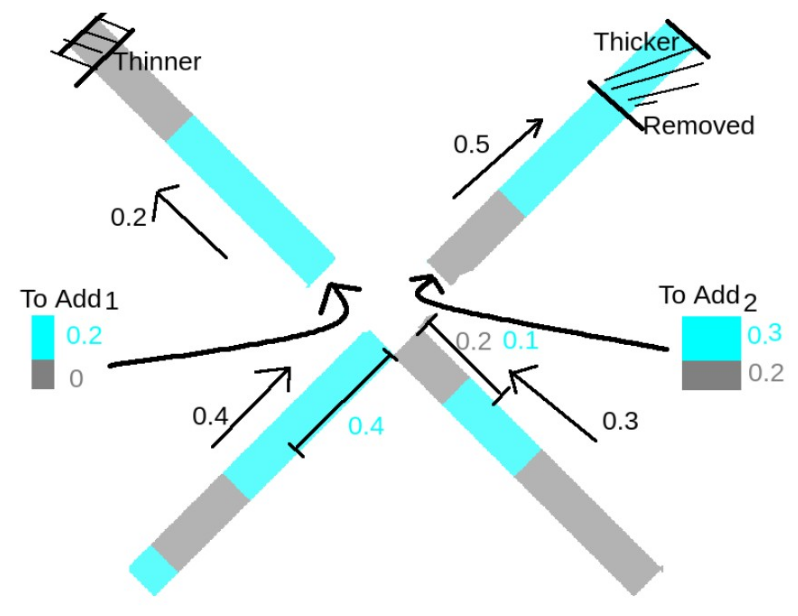
\includegraphics[width=0.48\textwidth]{fig_distributing_phases_intermediary}}
			\subfloat[Final tube configuration with 3 menisci. \label{fig:distributing_phases_final}]{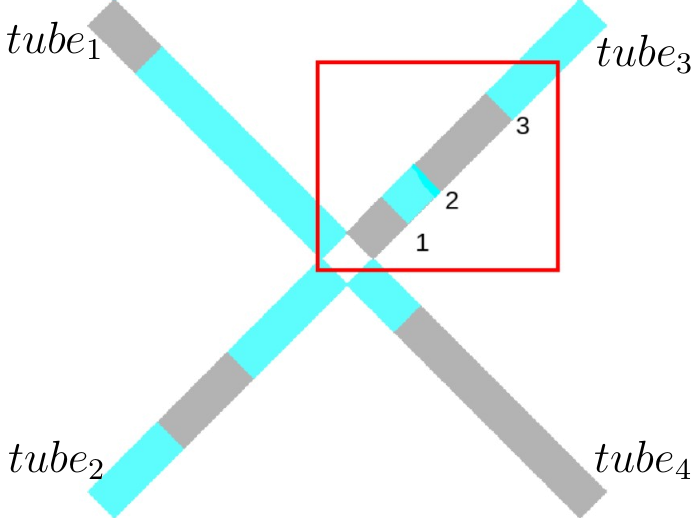
\includegraphics[width=0.42\textwidth]{fig_distributing_phases_final}}
			\caption{Occurrence of more than 2 menisci.}
		\end{figure}
		
		Step-2, we allocate this $0.5 u.V.$ of cyan fluid first into the thinner tube. The thinner ${tube}_1$ takes in $0.2 u.V.$. This allocation space is entirely filled by $0.2 u.V.$ of cyan fluid. Then for the thicker tube, we need to insert $0.5 u.V.$ of fluid into it. $0.3 u.V.$ of cyan fluid is inserted first then $0.2 u.V.$ of gray fluid.
				
		In figure \ref{fig:distributing_phases_final}, ${tube}_1$ retains the only meniscus because the end connected to the node initially contained cyan fluid, and we introduced $0.2 u.V.$ of more cyan fluid. The single meniscus was just displaced upwards.
		
		However, in ${tube}_3$, gray fluid was on the end of the tube connected to the node. We added $0.3 u.V.$ of cyan and $0.2 u.V.$ of gray fluid. Since the cyan fluid entered the thicker tube first, we end up with 3 menisci.	

	\subsection{Recombination} \label{sec:recombination-details}
		Our data structure was constrained to only allow the case for a maximum of two menisci in a tube. However, we see that in figure \ref{fig:distributing_phases_final} that there is possibility of more than 2 menisci occurring after distribution. We show the cases of distributing fluid in the nodes, which results in more than 2 menisci.
		
		\begin{figure}[H]
			\centering
			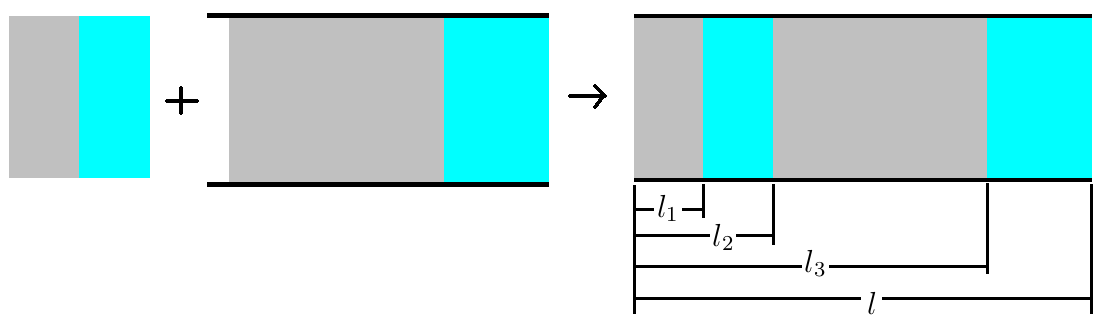
\includegraphics[width=0.8\textwidth]{fig_center-of-mass_1}
			\caption{Recombination of 3 menisci}
			\label{fig_center-of-mass_1}
		\end{figure}
		
		In figure \ref{fig_center-of-mass_1} we have a known amount of cyan and gray fluid which we need to insert into the tube. The tube which already consists of both the fluids. The flow is from left to right, so we insert the incoming fluids on the left end of the tube. Note that a block of cyan fluid always ends up in the center as it enters the tube first.
		
		Let $l_{i}$ denote the location of a meniscus. Since the tube is cylinder, the mass is simply proportional to the length they occupy in the tube, they are given by:
		
		\begin{gather}
			m_1 = l_2 - l_1 
		\end{gather}
		
		\begin{gather}
			m_2 = l - l_3
		\end{gather}
		
		Their respective center of masses $d_1$ and $d_2$ are given by:
		
		\begin{gather}	
			d_1 = \frac{l_1 + l_2}{2}
		\end{gather}
		
		\begin{gather}	
			d_2 = \frac{(l_3 + l)}{2}
		\end{gather}
		
		The center of mass of the cyan fluid in the tube is then given by:
		\begin{gather}
			d = \frac{m_1 d_1 + m_2 d_2}{m}
		\end{gather}
		
		Here,
		\begin{gather}
			m = m_1 + m_2
		\end{gather}
		
		
		We do not change the proportion of fluids in a tube during recombination. Therefore, it can be shown that if we recombine the fluids in a tube such that the center of mass of one of the fluid remained the same, then the center of mass of the other fluid will also remain the same.
		
		\begin{figure}[H]
			\centering
			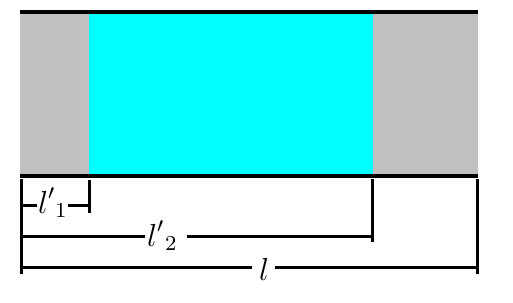
\includegraphics[width=0.4\textwidth]{fig_center-of-mass_final}
			\caption{After recombination, we always have 2 menisci}
		\end{figure}
		
		Let ${l'}_i$ denote the position of meniscus after recombination.
		
		\begin{gather}
			{l'}_1 = d - \frac{m}{2}
		\end{gather}
		
		\begin{gather}
			{l'}_2 = d + \frac{m}{2}
		\end{gather}
		

		\begin{figure}[H]
			\centering
			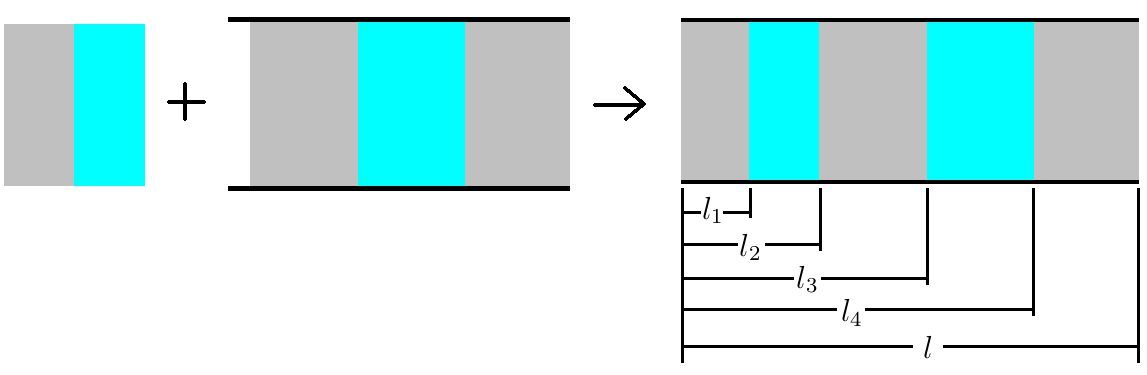
\includegraphics[width=0.9\textwidth]{fig_center-of-mass_2}
			\caption{Recombination of 4 menisci}
		\end{figure}
		
		When there are 4 menisci, we repeat the same process, except here:
		\begin{gather}
			m_2 = l_4 - l_3
		\end{gather}
		
		And
		
		\begin{gather}	
			d_2 = \frac{(l_3 + l_4)}{2}
		\end{gather}

	\subsection{Flow rate in a tube with one meniscus} \label{sec:simple-flow-rate}
		At first we derive the equation for flow rate when there is one meniscus present in a tube, then we generalize the case for $n$ menisci. The flow rate of a viscous fluid through a thin tube is given by the Hagen–Poiseuille equation:
		
		\begin{gather} \label{eq:flow-rate}
			Q = \frac{\pi}{8\mu} \frac{\Delta P}{l} R^4
		\end{gather}
		
		Here, $Q$ is the volumetric flow rate in $[m^3/s]$, $\Delta P$ is the pressure difference between the ends of the tube, $\mu$ is the viscosity in $[kg/m.s]$, $l$ is the length of the tube, $R$ is the radius of the tube.
		
		\begin{figure}[H]
			\centering
			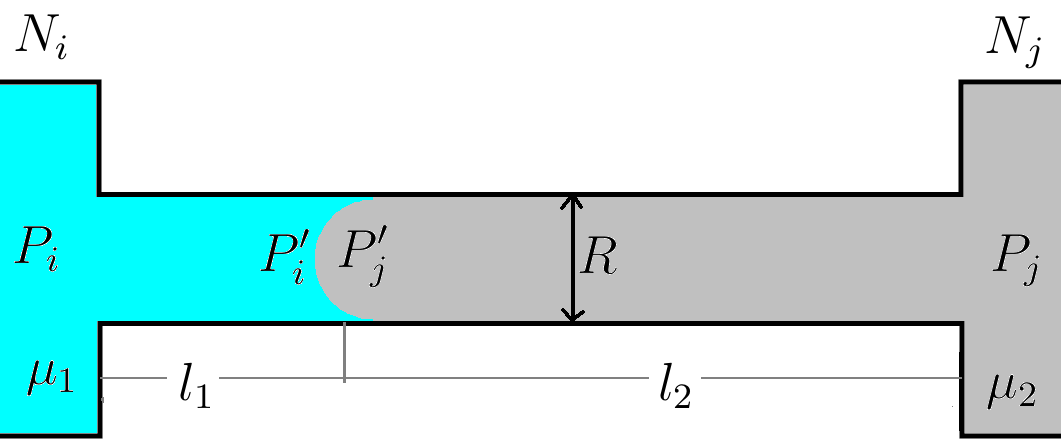
\includegraphics[height=3cm]{fig_capillary_pressure_in_tube_1mns_blue}
			\caption{Orientation of the meniscus, the convex side contains wetting fluid while the concave side contains non-wetting fluid.}
			\label{fig_capillary_pressure_in_tube_1mns_blue}
		\end{figure}
		
		In figure \ref{fig_capillary_pressure_in_tube_1mns_blue}, node $N_{i}$ kept at a pressure of $P_{i}$, and is filled with a wetting fluid of viscosity $\mu_{1}$. Node $N_{j}$ kept at a pressure of $P_{j}$ is filled with a non-wetting fluid of viscosity $\mu_{2}$. It is evident that the pressure on the convex size or on the part of the wetting fluid is lower.
		
		\begin{gather}
			P_{i}' < P_{j}'
		\end{gather}
		
		The pressure jump is given by:
		
		\begin{gather} \label{eq:capillary_pressure_mns}
			P_{j}' - P_{i}' = \frac{2 \sigma}{R}
		\end{gather}
		
		Here, $\sigma$ is the coefficient of surface tension in $[Pa.m]$ or $[kg/s]$.
		
		Separating figure \ref{fig_capillary_pressure_in_tube_1mns_blue} into two tubes of lengths $l_{1}$ and $l_{2}$, containing fluids of viscosity ${\mu}_1$ and ${\mu}_2$. The flow rates of the tubes, from equation \ref{eq:flow-rate} are given by:
		
		\begin{gather} \label{eq:flow-rate-first}
			Q = \frac{\pi}{8{\mu}_1} \frac{P_i - P^{'}_i}{l_1} R^4
		\end{gather}
		
		\begin{gather} \label{eq:flow-rate-second}
			Q = \frac{\pi}{8{\mu}_2} \frac{P^{'}_j - P_j}{l_2} R^4
		\end{gather}
		
		Due to the law of conservation of volume, the flow rates are equal. Adding the equations \ref{eq:flow-rate-first} and \ref{eq:flow-rate-second}:
		
		\begin{gather} \label{eq:flow-rate-intermediate}
			Q({\mu}_1 l_1 + {\mu}_2 l_2) = \frac{\pi}{8}R^4(P_i - P_j + P^{'}_j - P^{'}_i)
		\end{gather}
		
		Substituting the equation \ref{eq:capillary_pressure_mns} about capillary pressure,
		\begin{gather} \label{eq:flow-rate-1mns-basic-m}
			Q = \frac{\pi R^4}{8Ml} \left( \Delta P_{ij} + \frac{2\sigma}{R} \right)
		\end{gather}
		
		Here,
		\begin{gather} \label{eq:def-pressure-difference} 
			\Delta P_{ij} = P_{i} - P_{j}
		\end{gather}
		
		And $M$ is the viscosity parameter:
		\begin{gather}
			M = \sum_{k} \mu_{k} \frac{l_{k}}{l}
		\end{gather}
		Note that the viscosity parameter, remains the same for any number of menisci present in a tube.
		
		\subsection{Flow rate in a tube with multiple menisci} \label{sec:multi-menisci-flow-rate}
		\begin{figure}[H]
			\centering
			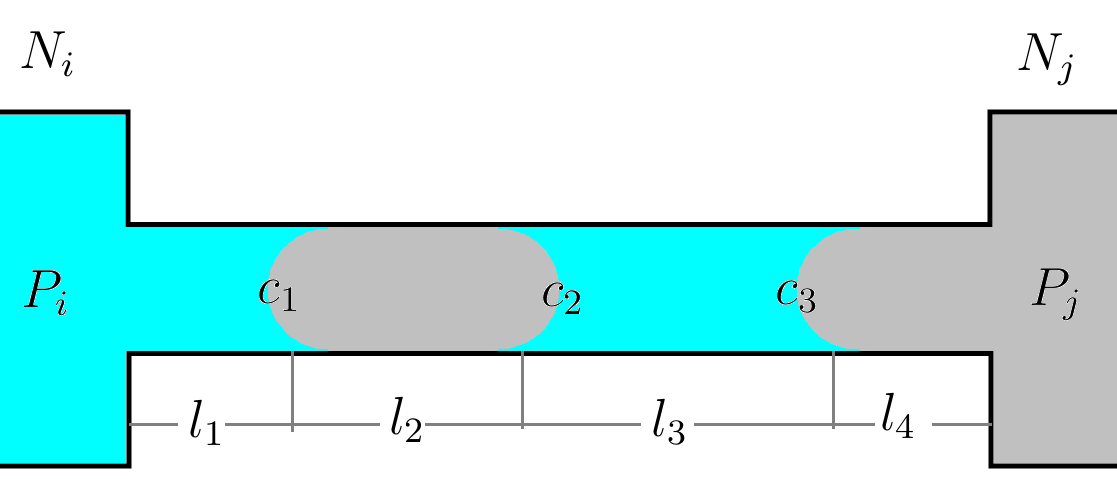
\includegraphics[height=3cm]{fig_capillary_pressure_in_tube_3mns}
			\caption{Capillary pressure contribution, $s = 1$}
			\label{fig:capillary_pressure_in_tube_3mns}
		\end{figure}
		
		Let the capillary pressures be denoted by the following:
		\begin{gather}
			c_1 = -c_2 = c_3 = \frac{2 \sigma}{R}
		\end{gather}
		
		Then for figure \ref{fig:capillary_pressure_in_tube_3mns}, the flow rate is given by:
		
		\begin{gather}
			Q = \frac{\pi R^4}{8Ml} \left( \Delta P_{ij} + c_1 + c_2 + c_3 \right)
		\end{gather}
		
		\begin{gather}
			Q = \frac{\pi R^4}{8Ml} \left( \Delta P_{ij} + \sum_{k} c_{k} \right)
		\end{gather}
		
		Flow rate for an arbitrary number of meniscus for a cylindrical tube, is given by:
		
		\begin{gather} \label{eq:main-flow-rate-with-s}
			\boxed{Q = \frac{\pi R^4}{8Ml} \left( \Delta P_{ij} + \frac{2s \sigma}{R} \right)}
		\end{gather}
		
		Where,
		
		\begin{gather} \label{eq:sign-func-def}
			s(d, n_{mns}) = 
			\begin{cases}
				-1,&\text{$n_{mns}$ = 1, $d$ points away from $N_{i}$}\\
				0,&\text{$n_{mns}$ = 0, 2}\\
				+1,&\text{$n_{mns}$ = 1, $d$ points towards $N_{i}$}
			\end{cases}
		\end{gather}
		
		Here,
		\begin{itemize}
			\item $d$, the direction the convex side of the meniscus points towards
			\item $n_{mns}$, the number of meniscus in a tube
		\end{itemize}
		
		In our model, the data structure does not accommodate more than 2 meniscus in a tube, hence in the definition of $s$, $n_{mns} \le 2$. Shown that, for figure \ref{fig:capillary_pressure_in_tube_3mns}, \ref{fig:capillary_pressure_in_tube_1mns_grey}, and \ref{fig:capillary_pressure_in_tube_2mns}, $s$ is $1$, $-1$, and $0$ respectively.
		
		\begin{figure}[H]
			\centering
			\subfloat[$s = -1$\label{fig:capillary_pressure_in_tube_1mns_grey}]{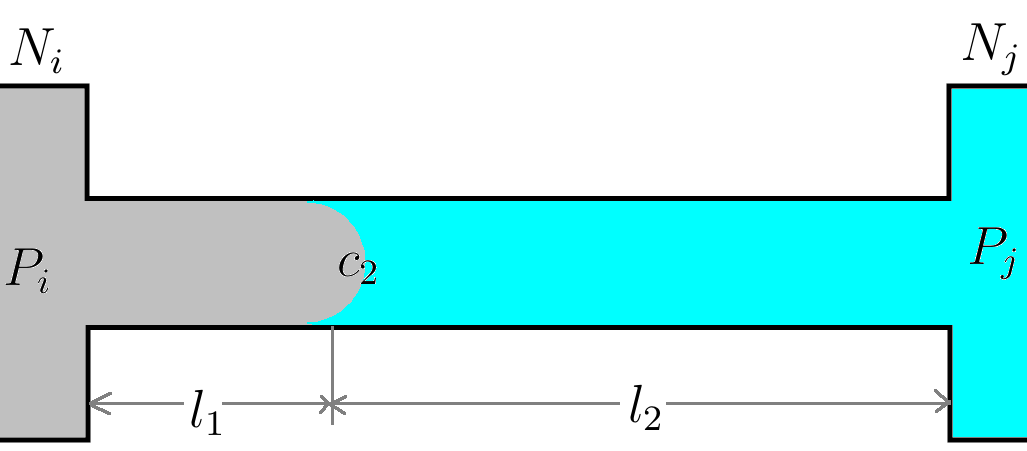
\includegraphics[width=0.45\textwidth]{fig_capillary_pressure_in_tube_1mns_grey}}
			\hfill
			\subfloat[$s = 0$ \label{fig:capillary_pressure_in_tube_2mns}]{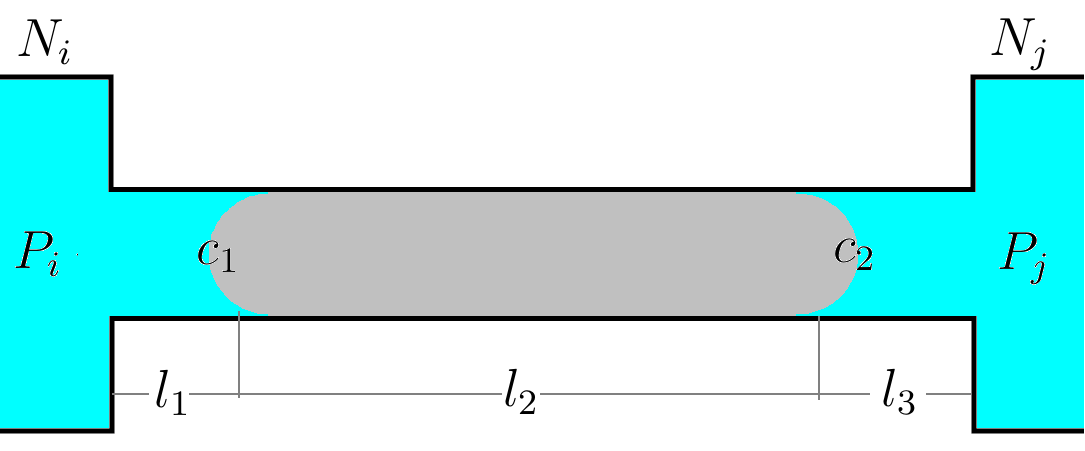
\includegraphics[width=0.48\textwidth]{fig_capillary_pressure_in_tube_2mns}}
			\caption{Capillary pressure contribution.}
		\end{figure}
		
	\subsection{Flow rate and velocity} \label{sec:flow-rate-vel}
		Therefore, in equation \ref{eq:flow-rate-simple-coeff}, we get:
		
		\begin{gather} \label{eq:flow-rate-aij}
			A_{ij} = \frac{\pi R_{ij}^4}{8M_{ij}l} \Delta P_{ij}
		\end{gather}
		
		\begin{gather} \label{eq:flow-rate-bij}
			B_{ij} = \frac{\pi R_{ij}^4}{8M_{ij}l} \frac{2 s_{ij} \sigma}{R_{ij}}
		\end{gather}
		
		Here, note that:
		\begin{gather}
			R_{ij} = R_{ji}
		\end{gather}
		
		\begin{gather}
			M_{ij} = M_{ji}
		\end{gather}
		
		\begin{gather}
			P_{ij} = -P_{ji}
		\end{gather}
		
		\begin{gather}
			s_{ij} = -s_{ji}
		\end{gather}
		
		It clear that:
		\begin{gather} \label{eq:symmetry-of-a}
			A_{ij} = A_{ji}
		\end{gather}
		
		\begin{gather} \label{eq:symmetry-of-b}
			B_{ij} = -B_{ji}
		\end{gather}
		
		When the pressures are known in each nodes, the velocity is determined by:
		\begin{gather} \label{eq:velocity-from-pressures}
			v_{ij} = \frac{Q_{ij}}{\pi R_{ij}^2} = \frac{R_{ij}^2}{8M_{ij}l} \left( \Delta P_{ij} + \frac{2s_{ij} \sigma}{R_{ij}} \right)
		\end{gather}
		
		[COMMENT: Not satisfied, in Pousielle's flow, the flow on the boundary is 0, and maximum in the center, how do we reason for selecting $v = Q/ \pi R^2$?]

		
	\section{Methods and examples of simulation} \label{sec:computation}	
		\subsection{Algorithm for the simulation} \label{sec:detailed-algorithm}
			\begin{enumerate}
				\item \textbf{Input constants:} declare ${\mu}_{1}$, ${\mu}_{2}$, $l$, $\sigma$.
				
				\item \textbf{Input files:} read radius and meniscus distribution.
				
				\item \textbf{Random radius:} add very small random values to the radius distribution, so that there is an unique way of distributing fluids into the tubes.
				
				\item \textbf{Create pressure matrix:} create a 0 filled augmented matrix $M_{ij}$ of $n$ rows and $n + 1$ columns, where $n$ is the number of nodes in our system, this matrix will be solved to find the pressures in each node.
				
				\item \textbf{Set time:} set the physical time of our simulation $t = 0$.
				\item \textbf{Main loop:} until a certain saturation $S$ is reached in a given region, or for a fixed number of frames:
				\begin{enumerate}
					\item \textbf{Generate linear equations:} iterate for every $N_i$, $1 \le i \le n$:
					
					\begin{enumerate}
						\item \textbf{Generate connections:} the list of nodes $N_j$ and tubes $b_{ij}$, which are connected to $N_i$.
						
						\item \textbf{Iterate connections:} for each node $N_j$ connected to $N_i$:
						
						\begin{enumerate}
							\item $R_{ij}$ is obtained from radius distribution. Calculate $M_{ij}$ and $s_{ij}$ from current meniscus configuration of $b_{ij}$.
							
							\item Using $R_{ij}$, $M_{ij}$, $s_{ij}$, and other constants, calculate $A_{ij}$ and $B_{ij}$ according to equations \ref{eq:flow-rate-aij} and \ref{eq:flow-rate-bij}.
							
							\item Perform the following modifications to $M_{ij}$:
							
							$M_{ii} = M_{ii} + A_{ii}$
							
							$M_{ij} = M_{ij} - A_{ij}$
							
							$M_{i,n + 1} = M_{i,n + 1} - B_{ij}$
						\end{enumerate}
					\end{enumerate}
					
					\item \textbf{Calculate pressures:} solve $M_{ij}$. Gaussian-elimination was used for the results of simulations shown in this article.
					
					\item \textbf{Calculate velocity:} from the pressures calculated in each node, determine the velocity in each tube using equation \ref{eq:velocity-from-pressures}.
					
					\item \textbf{Calculate time step:} the time step for integration $\Delta t = min(\Delta t_{ij})$, here $\Delta t_{ij} = c_{t} min(l/v_{ij})$ for each tube $b_{ij}$. $c_{t} = 0.1$ was used for the simulations.
					
					\item \textbf{Calculate volume displacement}, the volume displaced in each tube is determined by, $V_{ij} = v_{ij} \Delta t$.
					
					\item \textbf{Store distribution:} iterate through each tube, and store how much of which fluid enters into the node towards which there is positive velocity.
					
					\item \textbf{Integration:} iterate through all the nodes, and for each node $N_i$: 
					
					\begin{enumerate}
						\item \textbf{List outflow tubes:} determine which tubes take away fluid from $N_i$.
						
						\item \textbf{Distribute} the wetting and non-wetting fluids according to the algorithm described in \ref{sec:multi-phase-flow}.
						
						\item \textbf{Recombine} when a tube has more than 2 menisci, according to \ref{sec:recombination-details}.
					\end{enumerate}
						
					\item \textbf{Picture:} save a picture of the current configuration.
					
					\item \textbf{Update saturation:} calculate the new saturation $S$.
					
					\item \textbf{Update time:} $t = t + \Delta t$.
					
					\item \textbf{Add plot point:} add $(t, S)$ to the plot.
				\end{enumerate}
				
				\item \textbf{Video:} a video file is generated from the pictures.	
			\end{enumerate}

				
		\subsection{Modeling simple filtration: open boundaries} \label{sec:model-filtration}
			In a system with closed boundaries, no fluid can enter or leave the system. For the whole system, we have:
			
			\begin{gather}
				\frac{\partial S}{\partial t} = 0
			\end{gather}
			
			In a system with open boundaries, there is at least one node, into which fluid is externally added, and at least one node through which fluid leaves.
			
			Figure \ref{fig:simple-5-nodes} is an example of a system with open boundaries. We use open boundaries to test filtration. The nodes though which any amount of fluid can enter or leave is maintained at constant pressure.
			
			
			\begin{figure}[H]
				\centering
				\subfloat[Initial, wetting fluid confined to the bottom. \label{fig:plot-sat-vs-time-disp-one}]{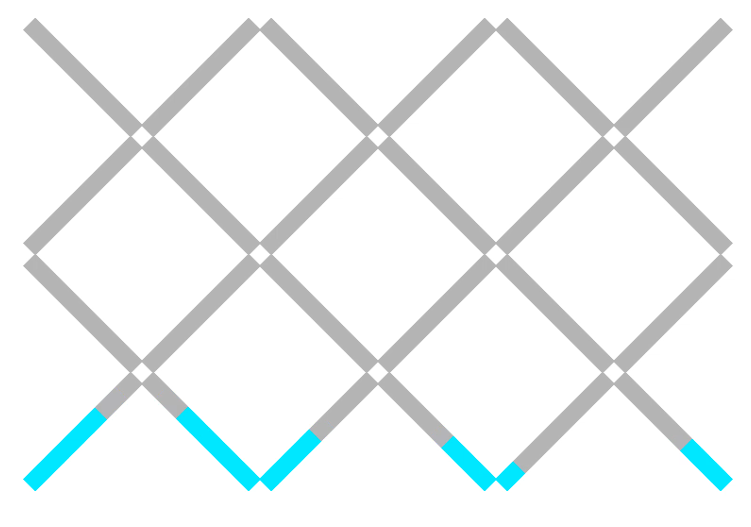
\includegraphics[width=0.47\textwidth]{fig_initial-fill-distribution}}
				\subfloat[Filtration with open boundaries. \label{fig:plot-sat-vs-time-disp-two}]{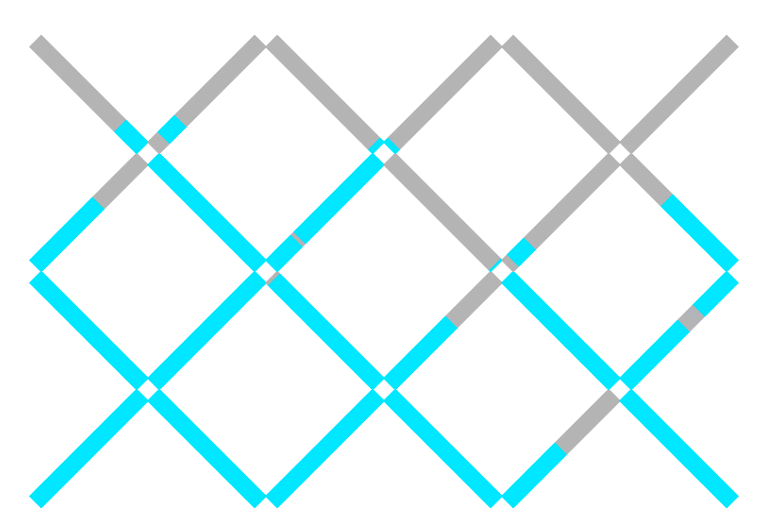
\includegraphics[width=0.47\textwidth]{fig_final-fill-distribution}}
				\caption{Filtration}
			\end{figure}
				
			Figure \ref{fig:plot-sat-vs-time-disp-one} consists of radius different thickness. A higher pressure is fixed for all nodes in the bottom layer, while a low pressure is fixed for the top row.

			
		\subsection{Solution for closed boundaries} \label{sec:closed-boundary-triangle}

			In an open system, the matrix is of the form \ref{eq:matrix-open-sys-5-nodes}, and an unique solution always exists. However we will now show that the set of linear equations for a system with closed boundaries has infinitely many solutions.

			\begin{figure}[H]
				\centering
				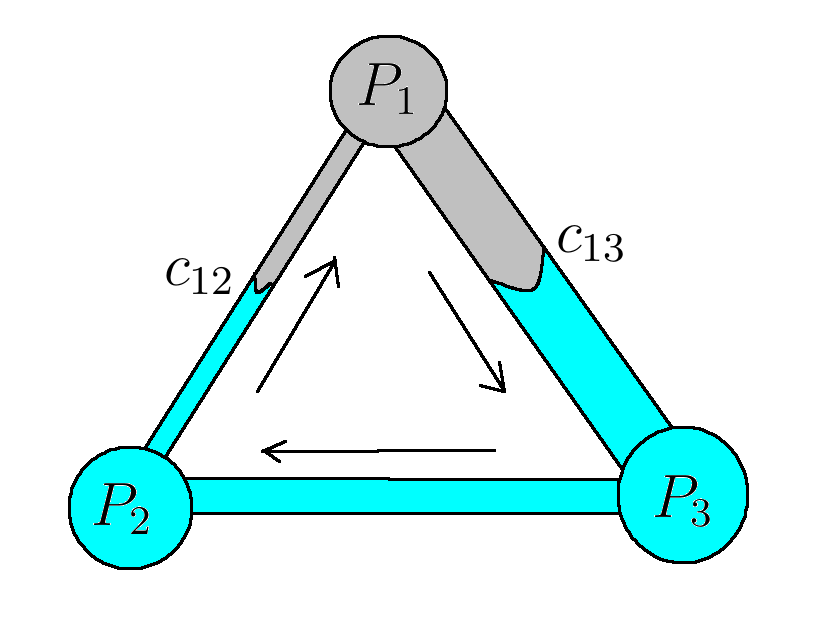
\includegraphics[height=4cm]{fig_zero-linearequation}
				\caption{Infinitely many solutions for a system with 3 nodes.}
				\label{fig:zero-la-triangle}
			\end{figure}
			
			The flow rates for $N_{1}$, according to equation \ref{eq:flow-rate-simple-coeff}:
			\begin{gather}
				Q_{12} = A_{12}(P_1 - P_2) + B_{12}
			\end{gather}
			
			\begin{gather}
				Q_{13} = A_{13}(P_1 - P_3) + B_{13}
			\end{gather}
			
			Due to conservation of volume:
			\begin{gather}
				Q_{12} + Q_{13} = 0
			\end{gather}
			
			So, we obtain:
			\begin{gather}
				(A_{12} + A_{13})P_1 - A_{12}P_2 - A_{13}P_3 = -B_{12} - B_{13}
			\end{gather}
			
			Applying the same for $N_2$ and $N_3$, we obtain the augmented matrix:
			\begin{gather}
				\begin{pmatrix}
					(A_{12} + A_{13}) & -A_{12} & -A_{13} & -B_{12} - B_{13} \\
					-A_{21} & (A_{21} + A_{23}) & -A_{23} & -B_{21} - B_{23} \\
					-A_{31} & -A_{32} & (A_{31} + A_{32}) & -B_{31} - B_{32} \\
				\end{pmatrix}
			\end{gather}
			
			From equation \ref{eq:symmetry-of-b}, we have $B_{ij} = -B_{ji}$. So, the sum of all columns are zeros.
				
			After applying $R_3 = R_3 + R_1 + R_2$ to the matrix:
			
			\begin{gather}
				\begin{pmatrix}
					(A_{12} + A_{13}) & -A_{12} & -A_{13} & -B_{12} - B_{13} \\
					-A_{21} & (A_{21} + A_{23}) & -A_{23} & -B_{21} - B_{23} \\
					0 & 0 & 0 & 0 \\
				\end{pmatrix}
			\end{gather}
			
			We obtain a zero row. This problem is solved by adding a constant $a$ to one of the column of the matrix for every row. 
			\begin{gather}
				\begin{pmatrix}
					(A_{12} + A_{13}) & -A_{12} & -A_{13} + a & -B_{12} - B_{13} \\
					-A_{21} & (A_{21} + A_{23}) & -A_{23} + a & -B_{21} - B_{23} \\
					-A_{31} & -A_{32} & (A_{31} + A_{32}) + a & -B_{31} - B_{32} \\
				\end{pmatrix}
			\end{gather}
			
			This is the general case, when we have an arbitrary configuration of capillary pressures. In figure \ref{fig:zero-la-triangle}, $B_{21} = c_{12}, B_{13} = -c_{13}, B_{32} = 0$. Now, after $R_3 = R_3 + R_1 + R_2$:
			\begin{gather}
				\begin{pmatrix}
					(A_{12} + A_{13}) & -A_{12} & -A_{13} + a & -B_{12} - B_{13} \\
					-A_{21} & (A_{21} + A_{23}) & -A_{23} + a & -B_{21} - B_{23} \\
					0 & 0 & 3a & 0 \\
				\end{pmatrix}
			\end{gather}
			
			\begin{gather}
				3aP_3 = 0
			\end{gather}
			
			The solution exists only if $P_3 = 0$. This is point of zero pressure. In our simulation, the center was chosen to be the point of zero pressure. Changing this point does not change the flow rates or the nature of flows.

		\subsection{Example of meniscus reaching a node: closed boundary} \label{sec:example-meniscus-in-node}
		
			\begin{figure}[H]
				\centering
				\subfloat[Showing radius thickness. \label{fig:plot-sat-vs-time-disp-one}]{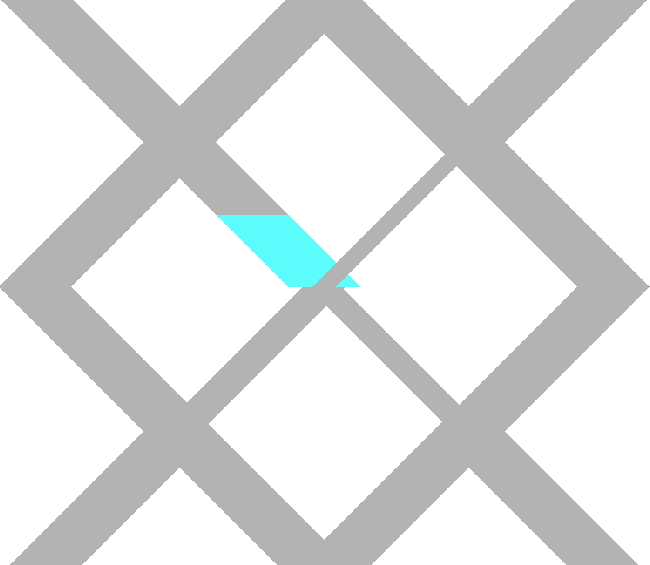
\includegraphics[width=0.42\textwidth]{fig_test_dist_th01}}
				\hfill
				\subfloat[Without showing thickness \label{fig:plot-sat-vs-time-disp-two}]{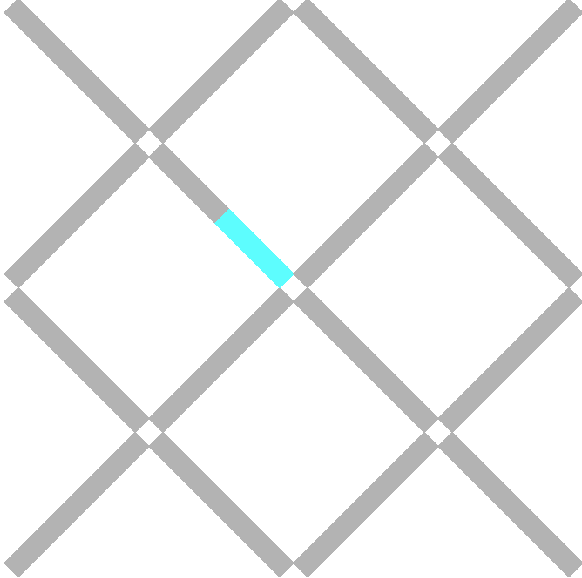
\includegraphics[width=0.40\textwidth]{fig_test_dist_tn01}}
				\caption{A meniscus just reached a node.}
			\end{figure}

			
			The tube where the cyan fluid is initially located is the thickest. After reaching the node, an additional 3 menisci are created very close to the node. Since the new tubes are all thinner than the initial. The capillary force from the new tubes is higher.
			
			\begin{figure}[H]
				\centering
				\subfloat[Showing radius thickness. \label{fig:plot-sat-vs-time-disp-one}]{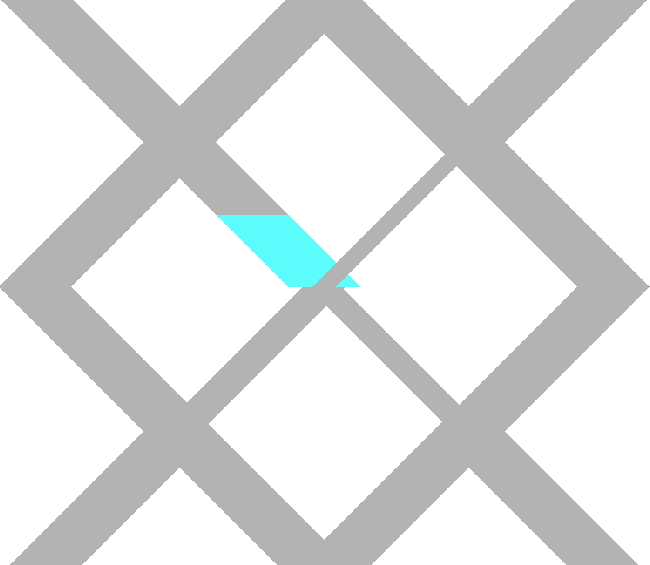
\includegraphics[width=0.42\textwidth]{fig_test_dist_th01}}
				\hfill
				\subfloat[Without showing thickness \label{fig:plot-sat-vs-time-disp-two}]{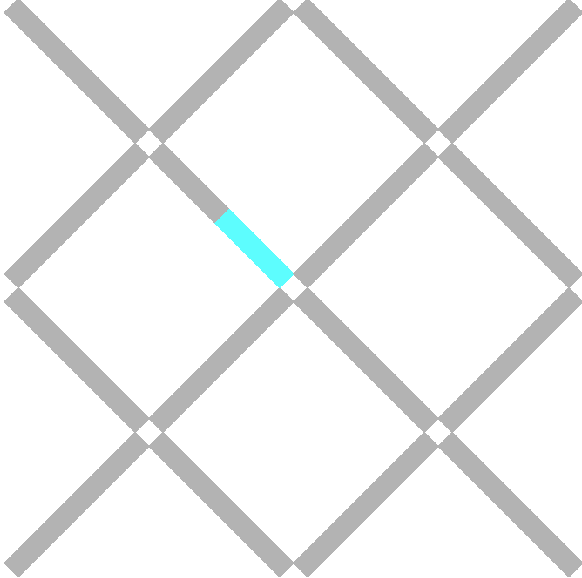
\includegraphics[width=0.40\textwidth]{fig_test_dist_tn01}}
				\caption{Cyan fluid being pulled by thinner tubes.}
			\end{figure}
			
			The thinnest tube pulls the cyan fluid away from the node the most, due to higher capillary pressure.	

	\section{Experiment and results} \label{sec:experiment}
		\subsection{Objective and initial conditions} \label{sec:exp-init}
			\begin{figure}[H]
				\centering
				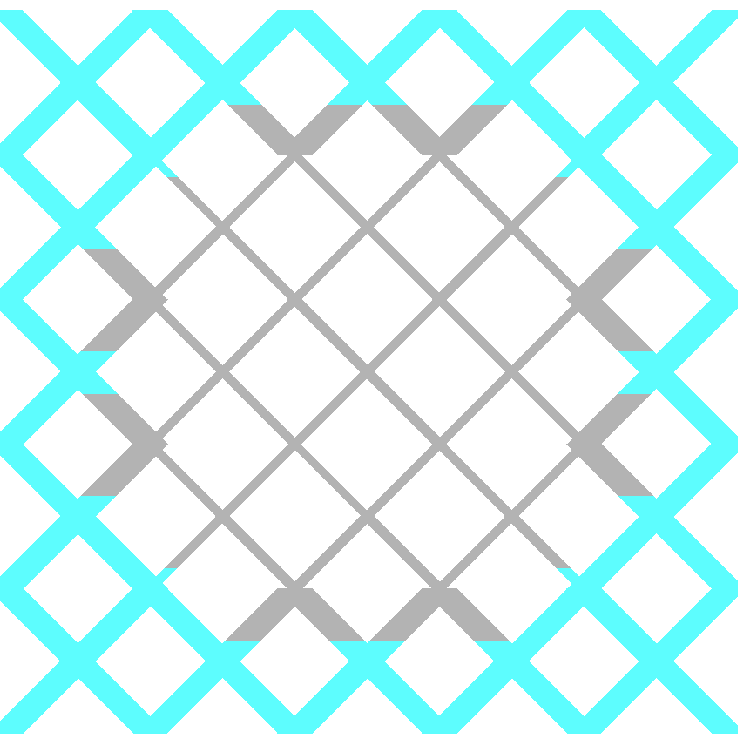
\includegraphics[height=8cm]{fig_result10by10_1}
				\caption{Initial setup example, non-wetting fluid initially located in the region with thinner radii.}
				\label{fig:invasion-result1}
			\end{figure}	
			
			Our objective is to model imbibition. In figure \ref{fig:invasion-result1}, all of the wetting fluid is located in the outer region, which has thicker radius. The inner region is filled with non-wetting fluid. In this simulation we wish to analyze the saturation of cyan fluid in the inner region with respect to time, $S = S(t)$. The features of the system are:
			
			\begin{itemize}
				\item The boundaries are closed.
				\item The radius in the outer region is 3 times larger, $R_{outer} = 3 * R_{inner}$.
				\item The size of the system is 26 x 26 tubes.
				\item Initially the volumes of wetting and non-wetting fluids in the whole system are equal. $V_{w} = V_{nw}$
			\end{itemize}
			
		\subsection{Experiment} \label{sec:exp-main}
			The algorithm was implemented in C++ 17, compiled using gcc 9.4.0. The computation was performed using processor 11th Gen Intel Core i5-1135G7 @ 2.40GHz operating with Ubuntu 20.04 LTS. The program was not paralleled, hence only one core of the processor was used at a time.  The simulation was done for 20,000 steps. Visualization of meniscus configuration and a plot point of saturation $S(t)$ was made for every 200 steps. It took about 1 minute to compile the whole program, and 5 minutes to simulate. If only the radius or initial meniscus configurations are changed, then recompiling is not required. The node located in the center of the system was chosen to have zero pressure. It was observed that changing the node which will have 0 pressure does not change the geometry of the flow.
			
			\begin{figure}[H]
				\centering
				\subfloat[Initial setup\label{fig:plot-sat-vs-time-disp-one}]{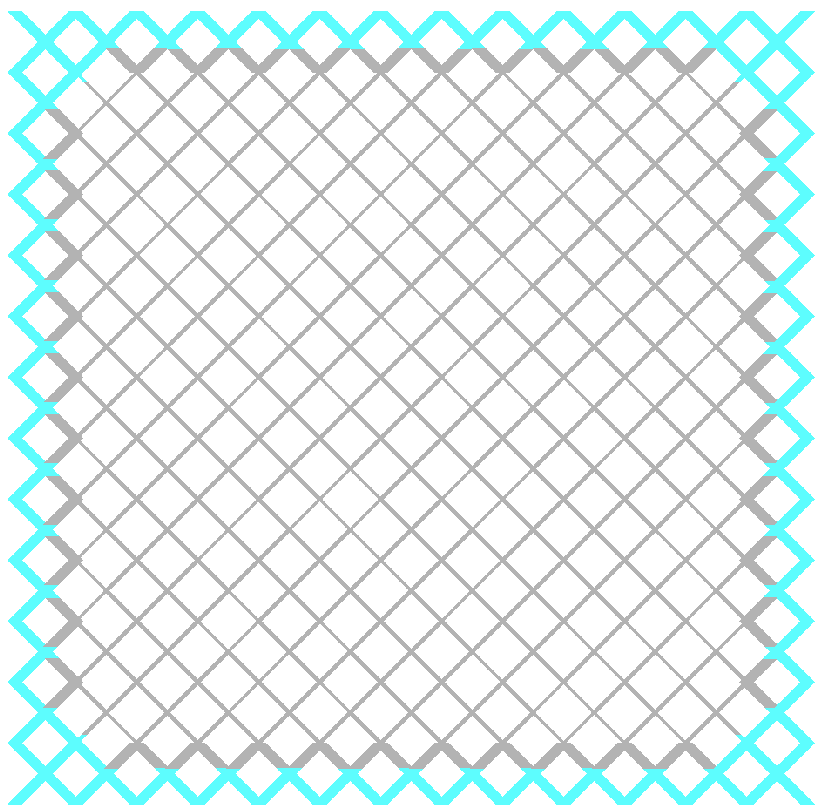
\includegraphics[width=0.46\textwidth]{fig_result26by26_1}}
				\hfill
				\subfloat[Final, in state of equilibrium \label{fig:plot-sat-vs-time-disp-two}]{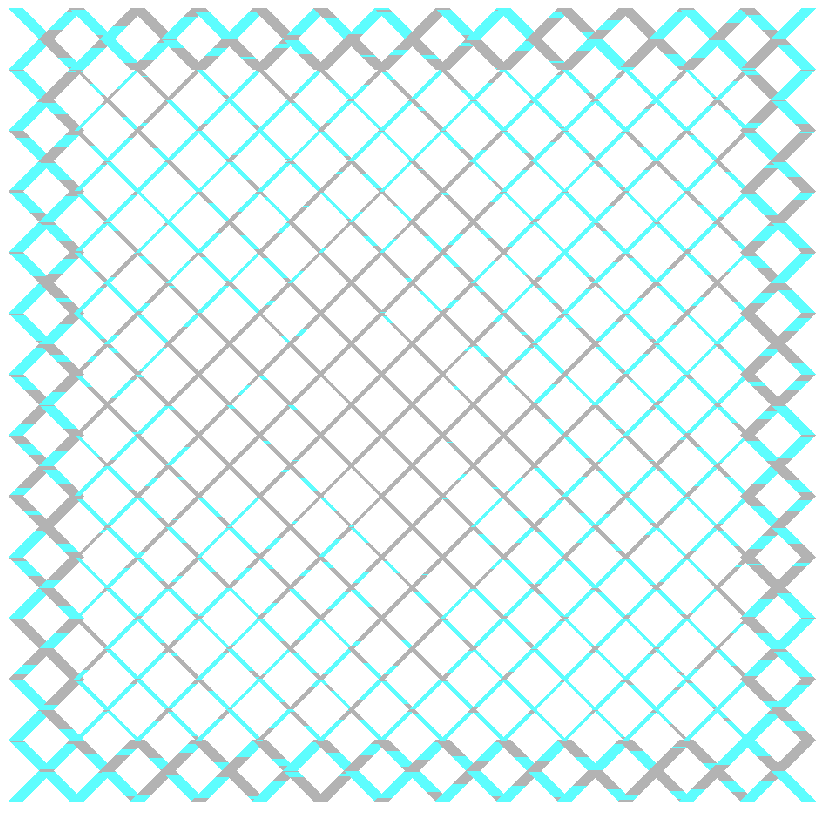
\includegraphics[width=0.46\textwidth]{fig_result26by26_4}}
				\caption{Plots of main experiment.}
			\end{figure}
			
			
			The plots are not symmetric because small random values $\Delta R / R ~ 10^{-3}$ was introduced to the system. The cyan fluid has invaded from the corners. We decided to plot for $26 x 26$ because a network model of this size can be easily simulated on a personal computer in a short time, and also it satisfies the conditions of gray and cyan fluids having about equal volumes, and the inner radius being 3 times thinner than the outer radius.
			
			The the part of the program slowing down the simulation is the solution of the linear equations using Gaussian-elimination. The process of Gaussian-elimination was not optimized. Hence, if we have $m$ variables, the time complexity for solution is $m^3$. If our network model is of size $n x n$ tubes, then the number of nodes is in the order of $n^2$. Therefore the time to compute grows with the size of the network model in the order of $n^6$. If we doubled the size of the network model, it would take $2^6 = 64$ times longer to perform the same simulation, which is about 5 hours on a personal computer, still reasonable time.
			
			For implementing the algorithm, $double$ is recommended over $float$. $float$ was earlier used to speed up the process by about $2$ times, however the errors grew significantly. The saturation is supposed to remain same due to closed boundaries, but it differed by as much as $10\%$ by the end of the simulation. The error in terms of volume of one of the fluid differing was less than $1\%$ when $double$ was used.
			
		\subsection{Discussion} \label{sec:exp-discussion}
			\begin{figure}[H]
				\centering
				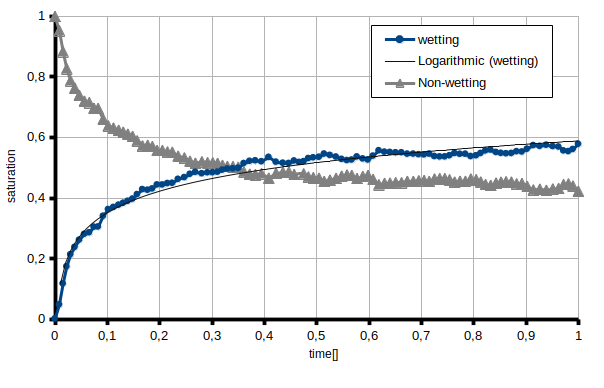
\includegraphics[width=1.0\textwidth]{fig_plot-sat-vs-time2}
				\caption{Plot of saturation of cyan fluid in inner region with respect to dimensionless time.}
			\end{figure}
			
			The equilibrium saturation for wetting fluid, $S_{eq} = 0.57$ for the inner region. For different viscosity ratio ${\mu}_1 / {\mu_2}$, the shape of the plot of $S(t)$ does not significantly differ. Changing constants of the experiment such as $\mu, \sigma, l$ simply changes the scale of the $x-axis$. Since the experiment was not calibrated to actual values, we decided to present our result in dimensionless time. It is obtained by simply diving the values on the $x-axis$ by the maximum.
			
			In in $S(t)$ plot of cyan fluid in the inner region. Initially the rate of invasion accelerates at a high rate, then the acceleration slows down, and finally the saturation reaches an equilibrium value which shows only irregular small oscillations. These irregular oscillations is expected to disappear on using a larger network model. They occur to the blocks of wetting fluid remaining in the outer region.
			
			The invasion of cyan fluid occurred from the corners, because in the corners each node is subjected to capillary forces more than from the middle of the edges. And the gray fluid was pushed out from the middle of the edges. The flow stops because of a large number of tubes ending up with 2 menisci. Tubes with two meniscus have a zero net capillary pressure, and cannot initiate flows. 
			
			$S(t)$ approximately shows a logarithmic dependence. It is clear that the relaxation parameter $\xi$ can be applied here the saturation converges to an equilibrium value. [Comment how to write the differential equation of Kondaurov.]


	\section{Conclusions} \label{sec:conclusion}
		\begin{enumerate}
		
			\item The novel method of distributing different fluids in the nodes, such the wetting fluid first goes into the tube with the thinner radius is valid, since it can model imbibition, where the saturation tends to an equilibrium value.
			
			\item The fact that the saturation $S(t)$ tends to an equilibrium value, implies that our network model can be used to simulate other relaxation phenomena, and it will help us better understand the physical meaning of the Kondaurov parameter $\xi$.
			
			\item The maximum number of connections a node in our network model can have is 4. Our algorithm can be easily extended to the more connections per node. Hence the same algorithm can be used to simulate a 3 dimensional network model.
			
			\item The fluctuations of $S(t)$, once the saturation reaches an equilibrium value is very small. Also the error in terms of fluid lost in a closed system is extremely small. The errors were extremely small because Gaussian-elimination was used to find the pressure in each node, which is more accurate than iterative methods.	
		\end{enumerate}
	
	\section{Appendix}
		The software can be found in https://github.com/kafiulshabbir/porus-fluid .
	
	\begin{thebibliography}{100}
		\bibitem[Aidun et al., 2010]{aidun2010lattice} \textit{Aidun, Cyrus K and Clausen, Jonathan R} Lattice-Boltzmann method for complex flows // Annual review of fluid mechanics, Annual Reviews.~--- 2010.~---  Vol.~42.~--- P.~439--472.

		\bibitem[Aker et al., 1998]{aker1998two} \textit{Aker, Eyvind and Jorgen Maaoy, Knut and Hansen, Alex and Batrouni, G George} A two-dimensional network simulator for two-phase flow in porous media // Transport in porous media, Springer.~--- 1998.~---  Vol.~32.~--- P.~163--186.

		\bibitem[Barenblatt et al., 1960]{barenblatt1960basic} \textit{Barenblatt, Grigory I and Zheltov, Iu P and Kochina, IN} Basic concepts in the theory of seepage of homogeneous liquids in fissured rocks [strata] // Journal of applied mathematics and mechanics, Pergamon.~--- 1960.~---  Vol.~24, No.~5.~--- P.~1286--1303.

		\bibitem[Barenblatt et al., 2003]{barenblatt2003mathematical} \textit{Barenblatt, GI and Patzek, TW and Silin, DB} The mathematical model of nonequilibrium effects in water-oil displacement // SPE journal, SPE.~--- 2003.~---  Vol.~8, No.~04.~--- P.~409--416.

		\bibitem[Bravo et al., 2008]{bravo2008analysis} \textit{Bravo, Maria C and Araujo, Mariela} Analysis of the unconventional behavior of oil relative permeability during depletion tests of gas-saturated heavy oils // International journal of multiphase flow, Elsevier.~--- 2008.~---  Vol.~34, No.~5.~--- P.~447--460.

		\bibitem[Chen et al., 1985]{chen1985pore} \textit{Chen, Jing-Den and Wilkinson, David} Pore-scale viscous fingering in porous media // Physical review letters, APS.~--- 1985.~---  Vol.~55, No.~18.~--- P.~1892.

		\bibitem[Chen et al., 1998]{chen1998lattice} \textit{Chen, Shiyi and Doolen, Gary D} Lattice Boltzmann method for fluid flows // Annual review of fluid mechanics, Annual Reviews 4139 El Camino Way, PO Box 10139, Palo Alto, CA 94303-0139, USA.~--- 1998.~---  Vol.~30, No.~1.~--- P.~329--364.

		\bibitem[Fatt, 1956]{fatt1956network} \textit{Fatt, I} The network model of porous media. 3. Dynamic properties of networks with tube radius distribution // Transactions of the American institute of mining and metallurgical engineers, MINERALS METALS MATERIALS SOC 420 COMMONWEALTH DR, WARRENDALE, PA 15086.~--- 1956.~---  Vol.~207, No.~7.~--- P.~164--181.

		\bibitem[Hassanizadeh et al., 1987]{hassanizadeh1987high} \textit{Hassanizadeh, S Majid and Gray, William G} High velocity flow in porous media // Transport in porous media, Springer.~--- 1987.~---  Vol.~2.~--- P.~521--531.

		\bibitem[Hassanizadeh et al., 1990]{hassanizadeh1990mechanics} \textit{Hassanizadeh, S Majid and Gray, William G} Mechanics and thermodynamics of multiphase flow in porous media including interphase boundaries // Advances in water resources, Elsevier.~--- 1990.~---  Vol.~13, No.~4.~--- P.~169--186.

		\bibitem[Hassanizadeh et al., 1993]{hassanizadeh1993thermodynamic} \textit{Hassanizadeh, S Majid and Gray, William G} Thermodynamic basis of capillary pressure in porous media // Water resources research, Wiley Online Library.~--- 1993.~---  Vol.~29, No.~10.~--- P.~3389--3405.

		\bibitem[Hassanizadeh et al., 2002]{hassanizadeh2002dynamic} \textit{Hassanizadeh, S Majid and Celia, Michael A and Dahle, Helge K} Dynamic effect in the capillary pressure--saturation relationship and its impacts on unsaturated flow // Vadose Zone Journal, Soil Science Society of America.~--- 2002.~---  Vol.~1, No.~1.~--- P.~38--57.

		\bibitem[Hassanizadeh, Majid, 2004]{hassanizadeh2004continuum} \textit{Hassanizadeh, S Majid} Continuum description of thermodynamic processes in porous media: Fundamentals and applications // Modeling Coupled Phenomena in Saturated Porous Materials.~--- 2004.~--- P.~179--223.

		\bibitem[Hubbert, King, 1956]{hubbert1956darcy} \textit{Hubbert, M King} Darcy's law and the field equations of the flow of underground fluids // Transactions of the AIME, SPE.~--- 1956.~---  Vol.~207, No.~01.~--- P.~222--239.

		\bibitem[Joekar-Niasar et al., 2010]{joekar2010non} \textit{Joekar-Niasar, V and Hassanizadeh, S Majid and Dahle, HK} Non-equilibrium effects in capillarity and interfacial area in two-phase flow: dynamic pore-network modelling // Journal of fluid mechanics, Cambridge University Press.~--- 2010.~---  Vol.~655.~--- P.~38--71.

		\bibitem[King, 1987]{king1987fractal} \textit{King, PR} The fractal nature of viscous fingering in porous media // Journal of Physics A: Mathematical and General, IOP Publishing.~--- 1987.~---  Vol.~20, No.~8.~--- P.~L529.

		\bibitem[Kondaurov, 2007]{kondaurov2007thermodynamically} \textit{Kondaurov, VI} The thermodynamically consistent equations of a thermoelastic saturated porous medium // Journal of applied mathematics and mechanics, Elsevier.~--- 2007.~---  Vol.~71, No.~4.~--- P.~562--579.

		\bibitem[Kondaurov, 2009]{kondaurov2009non} \textit{Kondaurov, VI} A non-equilibrium model of a porous medium saturated with immiscible fluids // Journal of Applied Mathematics and Mechanics, Elsevier.~--- 2009.~---  Vol.~73, No.~1.~--- P.~88--102.

		\bibitem[Konyukhov et al., 2019]{konyukhov2019homogenized} \textit{Konyukhov, Andrey and Pankratov, Leonid and Voloshin, Anton} The homogenized Kondaurov type non-equilibrium model of two-phase flow in multiscale non-homogeneous media // Physica Scripta, IOP Publishing.~--- 2019.~---  Vol.~94, No.~5.~--- P.~054002.

		\bibitem[Labed et al., 2012]{labed2012experimental} \textit{Labed, N and Bennamoun, L and Fohr, JP} Experimental study of two-phase flow in porous media with measurement of relative permeability // Fluid Dyn. Mater. Process, Citeseer.~--- 2012.~---  Vol.~8, No.~4.~--- P.~423--436.

		\bibitem[Raoof et al., 2010]{raoof2010new} \textit{Raoof, Amir and Hassanizadeh, S Majid} A new method for generating pore-network models of porous media // Transport in porous media, Springer.~--- 2010.~---  Vol.~81.~--- P.~391--407.

		\bibitem[Sinha et al., 2017]{sinha2017effective} \textit{Sinha, Santanu and Bender, Andrew T and Danczyk, Matthew and Keepseagle, Kayla and Prather, Cody A and Bray, Joshua M and Thrane, Linn W and Seymour, Joseph D and Codd, Sarah L and Hansen, Alex} Effective rheology of two-phase flow in three-dimensional porous media: experiment and simulation // Transport in porous media, Springer.~--- 2017.~---  Vol.~119.~--- P.~77--94.

		\bibitem[Tryggvason et al., 2001]{tryggvason2001front} \textit{Tryggvason, Gr{\'e}tar and Bunner, Bernard and Esmaeeli, Asghar and Juric, Damir and Al-Rawahi, N and Tauber, W and Han, J and Nas, S and Jan, Y-J} A front-tracking method for the computations of multiphase flow // Journal of computational physics, Elsevier.~--- 2001.~---  Vol.~169, No.~2.~--- P.~708--759.

		\bibitem[Uhlmann, Markus, 2005]{uhlmann2005immersed} \textit{Uhlmann, Markus} An immersed boundary method with direct forcing for the simulation of particulate flows // Journal of computational physics, Elsevier.~--- 2005.~---  Vol.~209, No.~2.~--- P.~448--476.

		\bibitem[Valvatne et al., 2004]{valvatne2004predictive} \textit{Valvatne, Per H and Blunt, Martin J} Predictive pore-scale modeling of two-phase flow in mixed wet media // Water resources research, Wiley Online Library.~--- 2004.~---  Vol.~40, No.~7.

		\bibitem[Washburn, Edward, 1921]{washburn1921dynamics} \textit{Washburn, Edward W} The dynamics of capillary flow // Physical review, APS.~--- 1921.~---  Vol.~17, No.~3.~--- P.~273.

	\end{thebibliography}
	
	
\end{document}
